\chapter{測地線、均勻加速度與牛頓極限}

眼前要處理的是重力。更確切地說，我們要找出描述近乎均勻重力場的時空度規，例如地球表面附近小型實驗室中的重力場。要得到這個度規，最直接的路徑反而不是直接求解。我們得先把三個幾何概念具體化：協變導數、平行移動與測地線運動。

這些概念彼此相依。協變導數告訴我們如何比較相鄰點的向量；平行移動告訴我們如何搬運向量而不使其轉向。若被搬運的向量就是路徑本身的切向量，便得到測地線。當路徑位於時空而非空間中時，同一個測地線方程也就成了自由落體粒子的運動方程。

講座後半段接著採取一個引人注目的做法：我們仍留在平坦的閔可夫斯基時空中，卻改用適用於一群剛性加速觀察者的座標來描述它。在這組座標中，度規看起來像是有重力。在一位觀察者附近，它重現均勻場的勢，而測地線滿足牛頓方程
\begin{equation}
\frac{d^2y}{d\tau^2}=-g.
\end{equation}
這就是以計算形式表述的等效原理。

\section{回顧協變導數}

在選定的點 \(P\)，可以選取盡可能接近笛卡兒座標的座標。講座一開始稱之為高斯法座標，隨即又加以限定。名稱不如局部條件重要：
\begin{equation}
g_{mn}(P)=\delta_{mn},
\qquad
\partial_r g_{mn}(P)=0.
\label{eq:l4-normal-point}
\end{equation}
這是在單一點上的法座標。它們不必在有限鄰域內維持笛卡兒形式；而且，由於座標軸可以旋轉，這類標架有許多種。

度規與導數算符相容：
\begin{equation}
\nabla_r g_{mn}=0,
\qquad
\nabla_r g^{mn}=0.
\label{eq:l4-metric-compatibility}
\end{equation}
對於協變向量 \(V_s\)，協變導數為
\begin{equation}
\nabla_r V_s
=
\partial_r V_s-\Gamma^p{}_{rs}V_p.
\label{eq:l4-covector-derivative}
\end{equation}
聯絡係數為
\begin{equation}
\Gamma^p{}_{rs}
=
\frac{1}{2}g^{pn}
\left(
\partial_s g_{nr}
+\partial_r g_{ns}
-\partial_n g_{rs}
\right).
\label{eq:l4-christoffel}
\end{equation}
講者在黑板上寫出這個式子時，修正了幾個指標。方程 \eqref{eq:l4-christoffel} 是修正後的完整關係。它對 \(r\) 與 \(s\) 對稱，這正是無撓的列維－奇維塔聯絡所預期的性質。

\begin{figure}[htbp]
\centering
\includegraphics[width=0.92\textwidth]{lecture_04_figure_01.png}
\caption{協變向量的導數與完整的克里斯托費爾符號公式。}
\end{figure}

克里斯托費爾符號由度規的一階導數構成，因此在座標 \eqref{eq:l4-normal-point} 中，它們於 \(P\) 處為零。即使底層空間是平坦的，它們在其他座標系中仍可能不為零。因此，\(\Gamma^p{}_{rs}\) 不是張量。這種非張量性正是加速觀察者能描述重力、而慣性觀察者看不到重力的原因。

\subsection{升起向量指標}

向量的相應導數不是另一條需要另外背下來的規則，而是由度規推得。先從
\begin{equation}
V^n=g^{np}V_p.
\end{equation}
開始，接著有
\begin{align}
\nabla_m V^n
&=\nabla_m\!\left(g^{np}V_p\right) \\
&=(\nabla_m g^{np})V_p+g^{np}\nabla_m V_p \\
&=g^{np}\left(\partial_mV_p-\Gamma^r{}_{mp}V_r\right),
\end{align}
其中第一項因度規相容性而消失。整理指標後得到
\begin{equation}
\nabla_m V^n
=
\partial_m V^n+\Gamma^n{}_{mr}V^r.
\label{eq:l4-vector-derivative}
\end{equation}

\begin{figure}[htbp]
\centering
\includegraphics[width=0.90\textwidth]{lecture_04_figure_02.png}
\caption{先以逆度規升起指標，再進行微分。}
\end{figure}

\begin{figure}[htbp]
\centering
\includegraphics[width=0.90\textwidth]{lecture_04_figure_03.png}
\caption{由度規相容性與乘積法則推得的上指標導數。}
\end{figure}

因此，指標的規則很簡單：
\begin{equation}
\boxed{
\begin{aligned}
\text{lower index:}&\quad -\Gamma,\\
\text{upper index:}&\quad +\Gamma.
\end{aligned}}
\end{equation}
對於高階張量，每個指標都會帶來一個聯絡項；正負號則由該指標是下標還是上標決定。

\subsection{術語問題}

上面提到的最佳座標究竟是什麼？這並不是在主張存在一組特別的全域座標系。在選定的一點上，這些座標使度規等於其平直形式，並使度規的一階導數為零。旋轉座標軸也會得到同樣合適的另一個標架。在這類標架中推得的幾何敘述不依賴座標軸的方向，因為最後得到的物理量是張量。

\section{沿曲線平行移動}

假設向量 \(V^n\) 沿著一條曲線移動。經過無窮小位移 \(dx^m\) 時，它的協變變化為
\begin{align}
\delta V^n
&=(\nabla_mV^n)\,dx^m \\
&=\partial_mV^n\,dx^m
+\Gamma^n{}_{mr}V^r\,dx^m \\
&=dV^n+\Gamma^n{}_{mr}V^r\,dx^m.
\label{eq:l4-covariant-differential}
\end{align}

\begin{figure}[htbp]
\centering
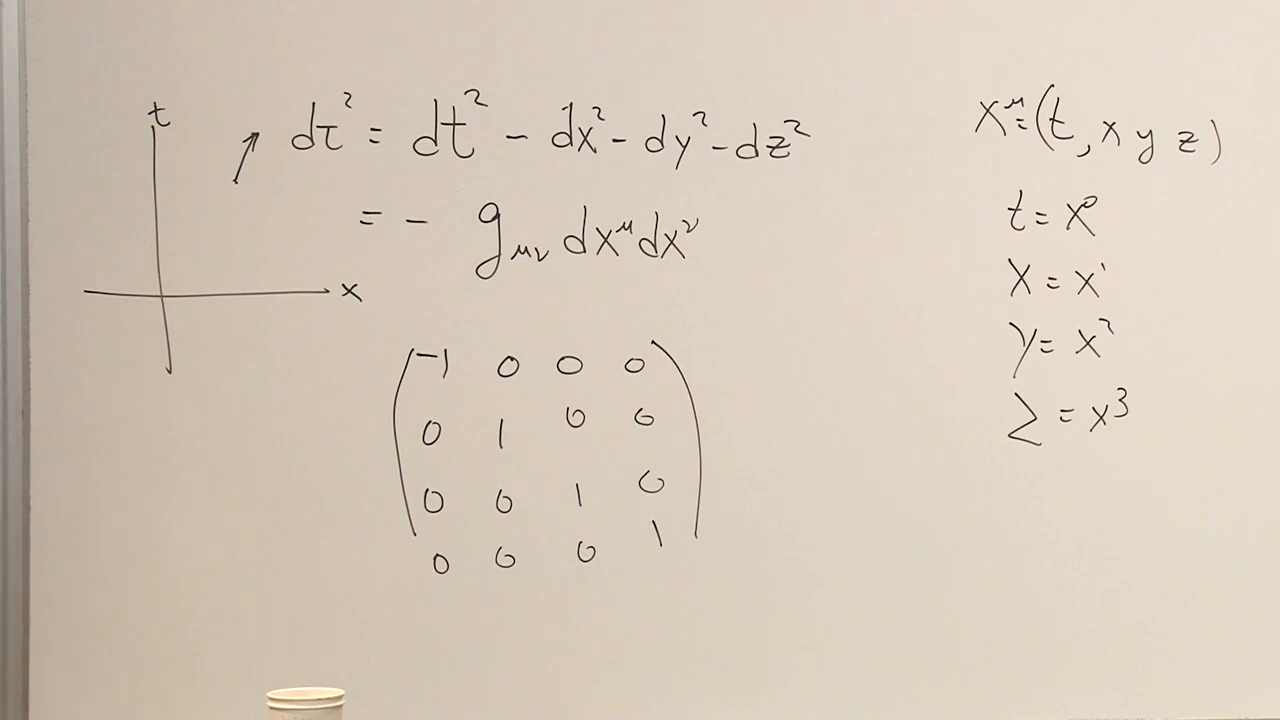
\includegraphics[width=0.92\textwidth]{lecture_04_figure_04.png}
\caption{沿曲線的分量變化與聯絡修正。}
\end{figure}

協變變化為零時，向量便是沿曲線平行移動：
\begin{equation}
\boxed{
dV^n+\Gamma^n{}_{mr}V^r\,dx^m=0.
}
\label{eq:l4-parallel-transport}
\end{equation}
從操作上來看，可以想像在曲線上的每一點都建立一個法標架。在該點的局部標架中，要求移動中的向量不轉向；接著前進一個無窮小距離，建立下一個法標架，再重複這個步驟。

\begin{figure}[htbp]
\centering
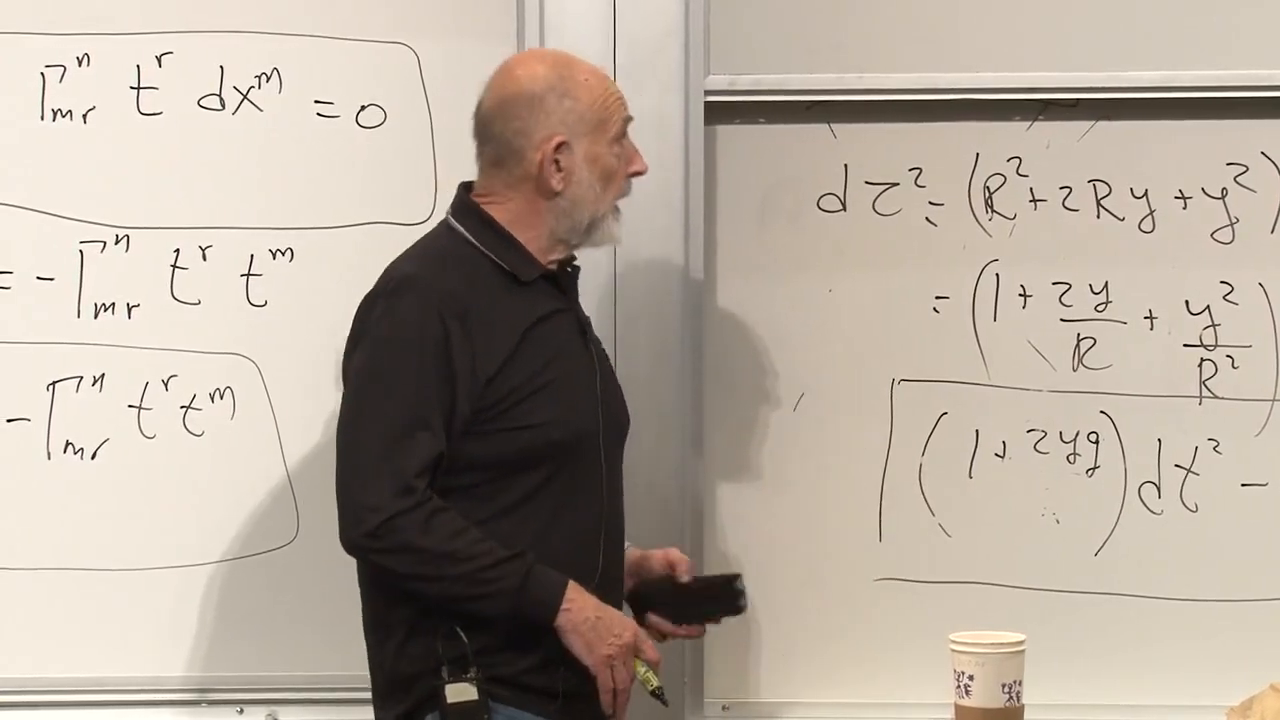
\includegraphics[width=0.92\textwidth]{lecture_04_figure_05.png}
\caption{平行移動方程的清楚板書。}
\end{figure}

每個臨時法標架的方向不屬於物理內容。比較之前，我們可以先旋轉標架。重要的是，協變敘述 \eqref{eq:l4-parallel-transport} 不受這項任意選擇影響。

\subsection{路徑依賴與曲率}

在彎曲空間中，平行移動會依賴路徑。從同一初始點上的同一向量出發，沿兩條不同路徑移動至同一終點，最後得到的向量一般會不同。向量沿閉合迴路移動一周後，可能會轉過一個角度。這種差異稱為整體性（holonomy），是曲率的直接表徵。

\begin{figure}[htbp]
\centering
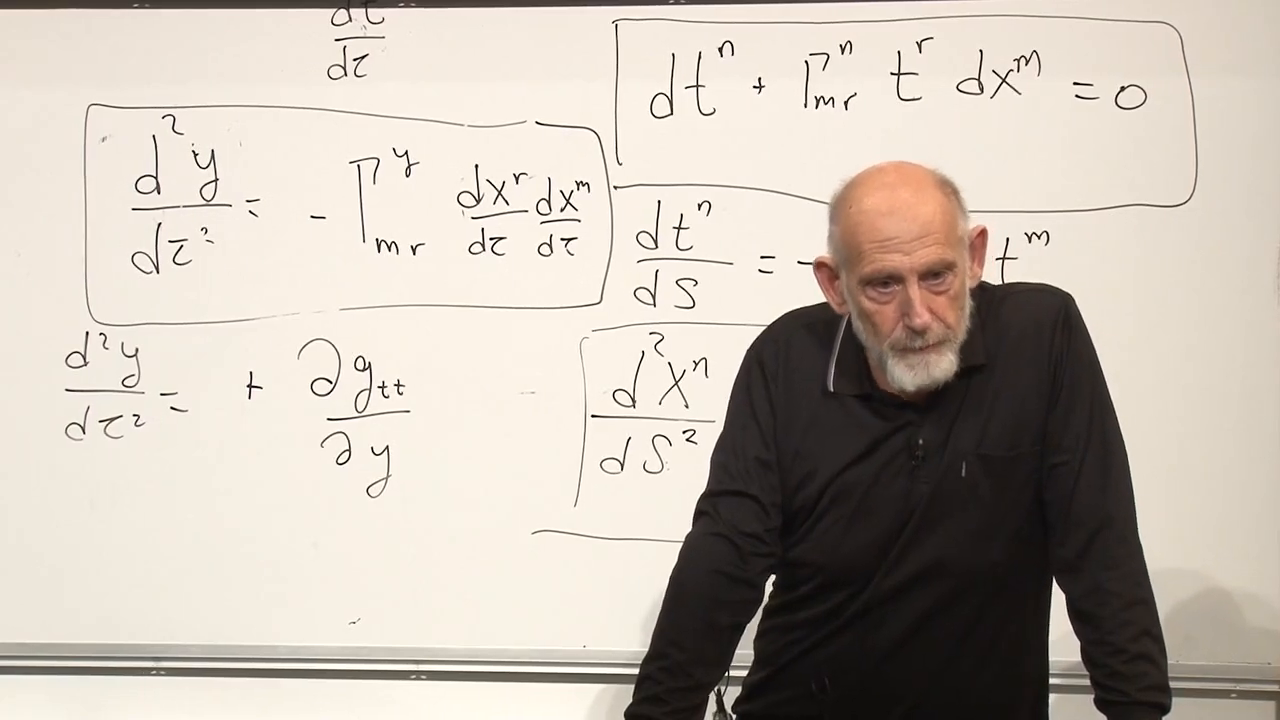
\includegraphics[width=0.90\textwidth]{lecture_04_figure_06.png}
\caption{在彎曲曲面上，沿兩條不同路徑平行移動向量，最後的方向不一定相同。}
\end{figure}

圓錐是個有用的例子。遠離頂點處，圓錐可以剪開並攤平。然而，若沿著包圍頂點的迴路平行移動向量，向量回到起點時仍會因角度虧損而轉過一個角度。若將頂點磨圓，曲率會是有限的，並分布在一小塊區域內；若頂點完全尖銳，理想化的情況就把曲率集中在頂點上。

\begin{figure}[htbp]
\centering
\includegraphics[width=0.90\textwidth]{lecture_04_figure_07.png}
\caption{圓錐上的圓周路徑，以及剪開攤平後的平面表示。}
\end{figure}

\subsection{關於平行移動向量的問題}

\paragraph{向量必須處處有定義嗎？}
不必。可以從單一點上的一個向量出發，只沿選定的曲線求解 \eqref{eq:l4-parallel-transport}；不一定要先定義完整的向量場。若已在某個區域定義向量場，它可能沿一個方向協變常數，沿另一個方向則不然。

\paragraph{向量的長度會保持不變嗎？}
會。令 \(V^2=g_{mn}V^mV^n\)。沿著曲線，
\begin{align}
\frac{D}{d\lambda}\left(g_{mn}V^mV^n\right)
&=
\frac{Dg_{mn}}{d\lambda}V^mV^n
+2g_{mn}V^m\frac{DV^n}{d\lambda}\\
&=0.
\end{align}
度規相容性使第一項消失，平行移動則使第二項消失。因此，平行移動會保留向量的長度與向量之間的夾角。

\paragraph{任意曲線的切向量都會平行移動嗎？}
不會。這個問題直接引出測地線。沿圓錐繞行的圓形路徑，其切向量會不斷轉向；將圓錐剪開攤平後形成的直線，其切向量則不會轉向。只有後者是局部直線。

\section{測地線：最直的路徑，不只是最短的路徑}

測地線有兩種相關的描述。從整體來看，它是長度或固有時泛函的駐值路徑。「駐值」一詞很重要：依幾何與端點而定，這條路徑不一定是唯一的全域最短路徑。在洛倫茲時空中，類時測地線在局部使固有時達到極大值，而非使某個正定距離達到極小值。

這裡需要的是局部描述。在彎曲地形上行駛的小車，若方向盤始終保持正向，就會描出一條測地線，前提是車子相對於地形彎曲的尺度夠小。這條路徑在嵌入空間中不一定看起來筆直；但依照曲面本身的幾何，它是直的。

\begin{figure}[htbp]
\centering
\includegraphics[width=0.90\textwidth]{lecture_04_figure_08.png}
\caption{在彎曲曲面上內在描繪的路徑，為「最直路徑」的定義作準備。}
\end{figure}

\subsection{切向量}

令曲線為 \(x^m(s)\)，其弧長為
\begin{equation}
ds^2=g_{mn}\,dx^m dx^n.
\end{equation}
單位切向量為
\begin{equation}
t^m=\frac{dx^m}{ds}.
\label{eq:l4-unit-tangent}
\end{equation}
從幾何上來看，取曲線上兩個相鄰的點，求出兩點間的位移向量，再除以兩點的間距，最後讓兩點逐漸重合。

\begin{figure}[htbp]
\centering
\includegraphics[width=0.90\textwidth]{lecture_04_figure_09.png}
\caption{切線方向是沿曲線取極限位移所得到的方向。}
\end{figure}

\begin{figure}[htbp]
\centering
\includegraphics[width=0.90\textwidth]{lecture_04_figure_10.png}
\caption{線元素與單位切向量 \(t^m=dx^m/ds\)。}
\end{figure}

測地線是切向量沿著自身平行移動的曲線：
\begin{equation}
dt^n+\Gamma^n{}_{mr}t^r\,dx^m=0.
\end{equation}
兩邊除以 \(ds\)，並使用 \(dx^m/ds=t^m\)：
\begin{equation}
\frac{dt^n}{ds}
=
-\Gamma^n{}_{mr}t^m t^r.
\end{equation}
最後代入 \(t^n=dx^n/ds\)：
\begin{equation}
\boxed{
\frac{d^2x^n}{ds^2}
+\Gamma^n{}_{mr}
\frac{dx^m}{ds}
\frac{dx^r}{ds}
=0.
}
\label{eq:l4-geodesic}
\end{equation}

\begin{figure}[htbp]
\centering
\includegraphics[width=0.94\textwidth]{lecture_04_figure_11.png}
\caption{切向量的平行移動定律與二階測地線方程。}
\end{figure}

方程 \eqref{eq:l4-geodesic} 已經很像牛頓動力學。若以適當的時間參數取代 \(s\)，第一項就是加速度。聯絡項則像單位質量所受的力，完全由度規決定。在廣義相對論中，這個類比成為實際的物理描述：自由粒子沿時空測地線運動，而牛頓所稱的重力加速度則透過聯絡項呈現。

\section{從黎曼距離到時空固有時}

討論現在從彎曲空間轉向時空。在慣性笛卡兒座標中，相鄰事件之間的固有時為
\begin{equation}
d\tau^2
=dt^2-dx^2-dy^2-dz^2.
\label{eq:l4-proper-time}
\end{equation}
講座採用
\begin{equation}
d\tau^2=-g_{\mu\nu}\,dx^\mu dx^\nu
\label{eq:l4-lecture-sign}
\end{equation}
其中
\begin{equation}
g_{\mu\nu}
=
\eta_{\mu\nu}
=
\begin{pmatrix}
-1&0&0&0\\
0&1&0&0\\
0&0&1&0\\
0&0&0&1
\end{pmatrix}.
\label{eq:l4-eta}
\end{equation}
因此，\eqref{eq:l4-lecture-sign} 中的外加負號，會將所選的 mostly-plus 度規轉換為 \eqref{eq:l4-proper-time}。座標為
\begin{equation}
\begin{aligned}
x^\mu&=(t,x,y,z),\\
x^0&=t,\quad x^1=x,\\
x^2&=y,\quad x^3=z.
\end{aligned}
\end{equation}

\begin{figure}[htbp]
\centering
\includegraphics[width=0.94\textwidth]{lecture_04_figure_12.png}
\caption{固有時、時空座標與 mostly-plus 閔可夫斯基度規。}
\end{figure}

號差是度規的不變資訊：一個本徵值具有時間方向的符號，另外三個則具有空間方向的符號。將整個度規乘以 \(-1\)，並一致地調整所有約定，就會得到同樣常用的 mostly-minus 約定。整體採用哪種約定不影響物理。

講座中有人問，是否考慮過其他不定號差的空間。在數學上，具有各種號差的偽黎曼幾何早已建立。物理上的重點較為有限：我們觀測到的相對論時空是洛倫茲型，只有一個時間方向。若增加時間方向，因果結構會有根本變化，也無法描述此處討論的物理。

\begin{figure}[htbp]
\centering
\includegraphics[width=0.94\textwidth]{lecture_04_figure_13.png}
\caption{在以 \(\eta_{\mu\nu}\) 表示平直度規之前，先確認符號約定。}
\end{figure}

平直時空不代表度規分量在所有座標系中都必須呈現為 \(\eta_{\mu\nu}\)；它只表示存在某些座標系，使度規分量呈現這種形式。即使黎曼張量為零，曲線座標或加速座標仍可能使度規分量隨位置改變。

\section{為什麼相同的座標加速度無法維持剛性}

我們想建立一套附著於加速電梯的座標。最初的想法是將一群觀察者以固定間距排列，並讓他們都具有相同的座標加速度。然而，相對論使這種直觀的安排無法維持剛性。

\begin{figure}[htbp]
\centering
\includegraphics[width=0.92\textwidth]{lecture_04_figure_14.png}
\caption{以一列相鄰觀察者檢驗共同加速度能否維持剛性。}
\end{figure}

若從某個慣性系來看，彼此分隔的觀察者遵循相同的加速程序，那麼在他們不斷改變的瞬時靜止系中，彼此間距就不會保持固定。連接他們的繩子會被拉長，最後斷裂。這與貝爾太空船思想實驗呈現的運動學張力相同。此外，牛頓式的定值座標加速度不可能無限持續，否則最終會預測出超過光速的速度。

因此，相對論中的剛性加速座標系必須讓不同位置的觀察者具有不同的固有加速度。越靠近預期視界的觀察者，加速度越大；越遠的觀察者，加速度越小。如此一來，他們之間的固有距離便能在瞬時共動系中保持固定。這就是一維空間中的玻恩剛性加速。

\section{以歐幾里得極座標暖身}

從一般的圓開始，最容易看清正確的構造。在歐幾里得平面中，
\begin{equation}
x=r\cos\theta,
\qquad
y=r\sin\theta,
\end{equation}
因此
\begin{equation}
x^2+y^2=r^2,
\qquad
\cos^2\theta+\sin^2\theta=1.
\end{equation}
複指數形式為
\begin{equation}
\cos\theta=\frac{e^{i\theta}+e^{-i\theta}}{2},
\qquad
\sin\theta=\frac{e^{i\theta}-e^{-i\theta}}{2i}.
\label{eq:l4-euler-trig}
\end{equation}
正弦公式分母中的 \(i\) 因子在講解時被發現漏寫，隨後補上。

\begin{figure}[htbp]
\centering
\includegraphics[width=0.94\textwidth]{lecture_04_figure_15.png}
\caption{圓、歐幾里得極座標，以及三角函數的複指數形式。}
\end{figure}

固定 \(r\) 的軌跡是一個圓。角速度固定時，向心加速度的大小固定，方向始終朝內。在時空中，雙曲線將扮演相應的角色。

\section{閔可夫斯基時空中的雙曲座標}

將三角函數換成相應的雙曲函數：
\begin{equation}
\cosh\omega=\frac{e^\omega+e^{-\omega}}{2},
\qquad
\sinh\omega=\frac{e^\omega-e^{-\omega}}{2},
\end{equation}
其中
\begin{equation}
\cosh^2\omega-\sinh^2\omega=1.
\label{eq:l4-hyperbolic-identity}
\end{equation}
這裡沒有 \(i\) 因子。座標 \(\omega\) 是雙曲角，也稱為快度。它不像一般角度那樣具有週期性；取值範圍從 \(-\infty\) 到 \(+\infty\)。

\begin{figure}[htbp]
\centering
\includegraphics[width=0.94\textwidth]{lecture_04_figure_16.png}
\caption{時空中的構造以雙曲函數取代圓函數。}
\end{figure}

在右側林德勒楔區中定義新座標：
\begin{equation}
x=r\cosh\omega,
\qquad
t=r\sinh\omega,
\qquad
r>0.
\label{eq:l4-rindler-transform}
\end{equation}
於是
\begin{equation}
x^2-t^2=r^2.
\label{eq:l4-rindler-hyperbola}
\end{equation}
固定 \(r\) 並改變 \(\omega\)，會描出一條雙曲線。增大 \(r\)，便沿類空方向穿過這一族雙曲線；增大 \(\omega\)，則沿著其中一條雙曲線朝類時方向前進。

\begin{figure}[htbp]
\centering
\includegraphics[width=0.94\textwidth]{lecture_04_figure_17.png}
\caption{座標變換 \(x=r\cosh\omega\)、\(t=r\sinh\omega\) 與不變的雙曲線方程。}
\end{figure}

\begin{figure}[htbp]
\centering
\includegraphics[width=0.94\textwidth]{lecture_04_figure_18.png}
\caption{一族固定 \(r\) 的雙曲線，代表一群剛性加速的觀察者。}
\end{figure}

\subsection{加速座標中的度規}

對 \eqref{eq:l4-rindler-transform} 微分：
\begin{align}
dx&=\cosh\omega\,dr+r\sinh\omega\,d\omega,\\
dt&=\sinh\omega\,dr+r\cosh\omega\,d\omega.
\end{align}
利用 \eqref{eq:l4-hyperbolic-identity}，交叉項會相消：
\begin{align}
d\tau^2
&=dt^2-dx^2\\
&=r^2\,d\omega^2-dr^2.
\label{eq:l4-rindler-metric}
\end{align}
恢復橫向方向後，只需在此處採用的固有時慣例中加上 \(-dy^2-dz^2\)。

這仍是平直時空。依賴座標的係數 \(r^2\)，並不比歐幾里得極座標中乘在 \(d\theta^2\) 前的 \(r^2\) 更能證明時空有曲率。

\subsection{雙曲線上的固有加速度}

對固定的世界線 \(r=R\)，方程 \eqref{eq:l4-rindler-metric} 給出
\begin{equation}
d\tau=R\,d\omega.
\end{equation}
其四維速度為
\begin{equation}
U^\mu
=
\frac{d(t,x)}{d\tau}
=
(\cosh\omega,\sinh\omega),
\end{equation}
四維加速度則為
\begin{equation}
A^\mu
=
\frac{dU^\mu}{d\tau}
=
\frac{1}{R}(\sinh\omega,\cosh\omega).
\end{equation}
其不變大小為常數：
\begin{equation}
a=\sqrt{A^\mu A_\mu}=\frac{1}{R}
\qquad (c=1).
\label{eq:l4-proper-acceleration}
\end{equation}

\begin{figure}[htbp]
\centering
\includegraphics[width=0.90\textwidth]{lecture_04_figure_19.png}
\caption{固定加速世界線的反半徑定律 \(a=1/R\)。}
\end{figure}

恢復單位後，
\begin{equation}
\boxed{a=\frac{c^2}{R}.}
\label{eq:l4-proper-acceleration-units}
\end{equation}

\begin{figure}[htbp]
\centering
\includegraphics[width=0.90\textwidth]{lecture_04_figure_20.png}
\caption{恢復單位後，\(1/R\)成為\(c^2/R\)。}
\end{figure}

截距 \(R\) 越小，世界線彎曲得越急，觀察者感受到的固有加速度也越大。位置更遠的雙曲線彎曲程度較小，所需加速度也較小。每位觀察者的加速度都不隨時間改變，但不同觀察者的加速度不同。正是這種差異使他們之間的固有距離得以保持不變。

\subsection{關於加速座標的問題}

\paragraph{\(R\)是 \(x\) 截距嗎？}
是。在 \(\omega=0\) 時，方程 \eqref{eq:l4-rindler-transform} 給出 \(t=0\) 與 \(x=R\)。截距透過 \eqref{eq:l4-proper-acceleration-units} 決定固有加速度。

\paragraph{這個構造是否取決於所選的原點？}
座標系會取決於原點。平移原點會得到另一族漸近線位置有所平移的雙曲線。這項選擇不影響任何不變的物理量。我們刻意選定一套加速座標系，並考察以這套座標描述慣性運動時會呈現什麼樣貌。

\paragraph{什麼是固有加速度？}
這是觀察者隨身攜帶的加速度計所測得的加速度。以協變形式表示：
\begin{equation}
A^\mu=\frac{dU^\mu}{d\tau},
\qquad
U^\mu=\frac{dx^\mu}{d\tau}.
\end{equation}
其大小代表觀察者實際感受到的推力，而不是遠方參考系指定的座標加速度 \(d^2x/dt^2\)。

\section{極座標與雙曲座標中的平直度規}

在聚焦於地球附近的局部區域之前，先並列歐幾里得與洛倫茲度規會很有幫助。在平面上，
\begin{equation}
ds^2=dr^2+r^2d\theta^2,
\qquad
g_{ab}
=
\begin{pmatrix}
1&0\\
0&r^2
\end{pmatrix}.
\label{eq:l4-polar-metric}
\end{equation}
有人提議加入球面因子，但這裡討論的是平面，不是球面。\(r^2\) 項記錄了這個事實：半徑越大，同一角度間隔所張成的弧越長。

\begin{figure}[htbp]
\centering
\includegraphics[width=0.94\textwidth]{lecture_04_figure_21.png}
\caption{歐幾里得極座標度規：平直平面中依賴位置的度規分量。}
\end{figure}

對應的閔可夫斯基度規為
\begin{equation}
d\tau^2=r^2d\omega^2-dr^2.
\end{equation}
兩個度規的分量都依賴位置，但兩種幾何仍然都是平直的。座標中的曲率與幾何曲率並非同一回事。

\section{聚焦地表加速度附近的局部區域}

選定一條固有加速度等於地表重力值 \(g\) 的參考雙曲線：
\begin{equation}
g=\frac{c^2}{R},
\qquad
R=\frac{c^2}{g}.
\label{eq:l4-earth-radius}
\end{equation}

\begin{figure}[htbp]
\centering
\includegraphics[width=0.94\textwidth]{lecture_04_figure_22.png}
\caption{以 \(c^2/R=g\) 選定參考雙曲線。}
\end{figure}

數值為
\begin{equation}
R
\simeq
\frac{(3.0\times10^8\ {\rm m\,s^{-1}})^2}
{9.8\ {\rm m\,s^{-2}}}
\simeq
9.2\times10^{15}\ {\rm m}.
\end{equation}
講座將這個數值約取為 \(10^{16}\) 公尺。相較於相對論尺度，一個地表重力加速度 \(g\) 很小，因此相應的林德勒半徑極大。

現在只看這位參考觀察者附近的一小塊區域。以 \(y\) 表示局部高度，定義為
\begin{equation}
r=R+y,
\qquad
dr=dy,
\qquad
|y|\ll R.
\label{eq:l4-local-height}
\end{equation}
講解時特別指出 \(dr=dy\)，因此空間項必須寫成 \(-dy^2\)。

代入 \eqref{eq:l4-rindler-metric}，得到
\begin{align}
d\tau^2
&=(R+y)^2d\omega^2-dy^2\\
&=(R^2+2Ry+y^2)d\omega^2-dy^2\\
&=
\left(
1+\frac{2y}{R}+\frac{y^2}{R^2}
\right)
R^2d\omega^2-dy^2.
\label{eq:l4-local-expand}
\end{align}

\begin{figure}[htbp]
\centering
\includegraphics[width=0.94\textwidth]{lecture_04_figure_23.png}
\caption{在 \(r=R+y\) 附近展開加速座標度規。}
\end{figure}

定義局部時間座標
\begin{equation}
t=R\omega.
\label{eq:l4-local-time}
\end{equation}
於是
\begin{equation}
d\tau^2
=
\left(
1+\frac{2y}{R}+\frac{y^2}{R^2}
\right)dt^2-dy^2.
\label{eq:l4-local-exact}
\end{equation}

\begin{figure}[htbp]
\centering
\includegraphics[width=0.94\textwidth]{lecture_04_figure_24.png}
\caption{在參考雙曲線附近展開後，引入 \(t=R\omega\)。}
\end{figure}

即使垂直移動幾十公里，相較於 \(R\) 仍然微不足道。講座以約二十四英里的下落距離作為具體例子：這樣的距離仍遠小於 \(10^{16}\) 公尺。因此，\(y^2/R^2\) 遠小於 \(y/R\)，可以略去二次項：
\begin{equation}
d\tau^2
\simeq
\left(1+\frac{2y}{R}\right)dt^2-dy^2.
\label{eq:l4-local-linear}
\end{equation}

\begin{figure}[htbp]
\centering
\includegraphics[width=0.94\textwidth]{lecture_04_figure_25.png}
\caption{弱場近似截斷前的度規展開與局部時間代換。}
\end{figure}

在 \(c=1\) 的單位制下，方程 \eqref{eq:l4-earth-radius} 給出 \(1/R=g\)，因此
\begin{equation}
\boxed{
d\tau^2\simeq(1+2gy)\,dt^2-dy^2.
}
\label{eq:l4-uniform-metric}
\end{equation}

\begin{figure}[htbp]
\centering
\includegraphics[width=0.94\textwidth]{lecture_04_figure_26.png}
\caption{均勻加速電梯的完整局部度規。}
\end{figure}

量
\begin{equation}
\Phi(y)=gy
\end{equation}
是均勻重力場中每單位質量的牛頓重力位勢。因此
\begin{equation}
d\tau^2\simeq(1+2\Phi)\,dt^2-dy^2
\qquad (c=1).
\label{eq:l4-weak-potential-propertime}
\end{equation}
按照講座採用的慣例 \(d\tau^2=-g_{\mu\nu}dx^\mu dx^\nu\)，這表示
\begin{equation}
g_{tt}=-(1+2\Phi).
\label{eq:l4-gtt-potential}
\end{equation}
在常用單位制中，無因次修正項為 \(2\Phi/c^2\)。

時空並沒有彎曲。方程 \eqref{eq:l4-uniform-metric} 是平坦林德勒度規在局部的展開。看似重力的效應，是加速電梯內觀察到的慣性力。

\section{測地線方程如何成為牛頓定律}

目前將 \(gy\) 認作位勢，還只是線索。決定性的檢驗在於動力學：度規 \eqref{eq:l4-uniform-metric} 中的自由粒子，是否會以 \(d^2y/dt^2=-g\) 向下加速？

對於以固有時為參數的類時世界線，
\begin{equation}
\frac{d^2x^\nu}{d\tau^2}
+\Gamma^\nu{}_{\mu\rho}
\frac{dx^\mu}{d\tau}
\frac{dx^\rho}{d\tau}
=0.
\label{eq:l4-spacetime-geodesic}
\end{equation}
其垂直分量為
\begin{equation}
\frac{d^2y}{d\tau^2}
=
-\Gamma^y{}_{\mu\rho}
\frac{dx^\mu}{d\tau}
\frac{dx^\rho}{d\tau}.
\label{eq:l4-y-geodesic}
\end{equation}

\begin{figure}[htbp]
\centering
\includegraphics[width=0.94\textwidth]{lecture_04_figure_27.png}
\caption{輸運方程及其二階測地線形式，可用來處理垂直運動。}
\end{figure}

\subsection{低速近似}

對於在弱靜態場中緩慢運動的粒子，
\begin{equation}
\frac{dt}{d\tau}\simeq1,
\qquad
\left|\frac{dy}{d\tau}\right|\ll1.
\end{equation}
因此，四維速度的時間分量量級為一，而空間分量相較之下很小。在 \eqref{eq:l4-y-geodesic} 的各項乘積中，主要貢獻來自 \(\mu=\rho=t\)：
\begin{equation}
\frac{d^2y}{d\tau^2}
\simeq
-\Gamma^y{}_{tt}
\left(\frac{dt}{d\tau}\right)^2
\simeq
-\Gamma^y{}_{tt}.
\label{eq:l4-slow-geodesic}
\end{equation}

\begin{figure}[htbp]
\centering
\includegraphics[width=0.94\textwidth]{lecture_04_figure_28.png}
\caption{將時空測地線方程套用於緩慢運動粒子的 \(y\) 分量。}
\end{figure}

現在計算所需的聯絡係數。度規是對角矩陣，且不依賴 \(t\)，因此
\begin{align}
\Gamma^y{}_{tt}
&=
\frac{1}{2}g^{yy}
\left(
\partial_tg_{yt}
+\partial_tg_{ty}
-\partial_yg_{tt}
\right)\\
&=
-\frac{1}{2}\partial_yg_{tt},
\label{eq:l4-gamma-ytt}
\end{align}
這是因為在講座採用的時間負、空間正號的張量慣例中，\(g^{yy}=1\)。

\begin{figure}[htbp]
\centering
\includegraphics[width=0.94\textwidth]{lecture_04_figure_29.png}
\caption{克里斯托費爾公式化簡為 \(y,t,t\) 分量。}
\end{figure}

合併 \eqref{eq:l4-slow-geodesic} 與 \eqref{eq:l4-gamma-ytt}，得到
\begin{equation}
\frac{d^2y}{d\tau^2}
\simeq
\frac{1}{2}\partial_yg_{tt}.
\label{eq:l4-accel-gtt}
\end{equation}
由 \eqref{eq:l4-gtt-potential}，
\begin{equation}
\partial_yg_{tt}
=
-2\partial_y\Phi
=
-2g.
\end{equation}
因此
\begin{equation}
\boxed{
\frac{d^2y}{d\tau^2}=-g.
}
\label{eq:l4-newton-result}
\end{equation}
在相同的低速近似下，\(t\simeq\tau\)，所以也可寫成
\begin{equation}
\frac{d^2y}{dt^2}=-g.
\end{equation}

\begin{figure}[htbp]
\centering
\includegraphics[width=0.94\textwidth]{lecture_04_figure_30.png}
\caption{完整的正負號推導：對 \(g_{tt}\) 取 \(y\) 導數，便得到加速度 \(-g\)。}
\end{figure}

更一般地，在牛頓近似下，
\begin{equation}
\boxed{
\begin{aligned}
g_{tt}&=-(1+2\Phi),\\
\frac{d^2x^i}{dt^2}&=-\partial_i\Phi
\end{aligned}
}
\qquad(c=1).
\label{eq:l4-newton-general}
\end{equation}
恢復單位後，度規修正為 \(2\Phi/c^2\)，加速度則仍為 \(-\boldsymbol{\nabla}\Phi\)。

這項計算說明了為何核心對象是度規，而不是額外引入的重力場。自由粒子只需沿時空測地線運動。在適用於加速實驗室的座標中，這條測地線會呈現出通常歸因於重力的座標彎曲。

\subsection{關於所選林德勒原點的問題}

能否平移參考雙曲線，讓它的漸近線與截距出現在其他位置？可以。每一個合適的平移原點，都對應一套均勻加速座標系。以電梯為例，這些選擇相當於指定電梯地板在某一瞬間所在的位置。

局部結果不仰賴某個特殊原點。選定固有加速度為 \(g\) 的參考觀察者後，\(y\) 就表示相對於該觀察者的高度，而附近的度規具有 \eqref{eq:l4-uniform-metric} 的形式。任意選擇座標系，只會決定我們將地板描述在何處，不會產生不變曲率。

\section{為什麼克里斯托費爾符號不是張量}

課後討論回到一個在回顧時首次提到的要點。在原本的慣性座標中，
\begin{equation}
g_{\mu\nu}=\eta_{\mu\nu},
\qquad
\partial_\rho\eta_{\mu\nu}=0,
\qquad
\Gamma^\mu{}_{\nu\rho}=0.
\end{equation}
自由粒子沿直線運動，不受重力。

在加速座標中，同一個平坦時空的度規分量會隨位置改變。克里斯托費爾符號不為零，因此同一條慣性軌跡看起來會彎曲，粒子彷彿正朝電梯地板落下。

若 \(\Gamma^\mu{}_{\nu\rho}\) 是張量，這種情況便不可能發生。在某個座標系中為零的張量，在所有座標系中都會是零。但聯絡在座標變換下會多出非齊次項，因此它可以在慣性系中為零、在加速系中不為零。這正是等效原理所要求的：
\begin{equation}
\text{accelerated frame}
\quad\longleftrightarrow\quad
\text{local gravity}.
\end{equation}

曲率的性質不同。黎曼張量是張量；若它在慣性系中為零，在加速系中也會為零：
\begin{equation}
R^\mu{}_{\nu\rho\sigma}=0.
\end{equation}
因此，克里斯托費爾符號描述的是依賴座標的重力效應；曲率則反映不因座標變換而消失的不變潮汐效應。

\section{從均勻位勢預覽史瓦西度規}

加速電梯中沒有造成重力的物質，也沒有曲率。不過，弱場關係 \eqref{eq:l4-newton-general} 提示我們，應如何考察實際球形質量產生的場。質量 \(M\) 外部的牛頓位勢為
\begin{equation}
\Phi(r)=-\frac{GM}{r}.
\label{eq:l4-newton-potential}
\end{equation}
將它代入弱場度規的時間分量，可得
\begin{equation}
g_{tt}
\simeq
-\left(1-\frac{2GM}{r}\right)
\qquad(c=1).
\label{eq:l4-schwarzschild-preview}
\end{equation}
講解時修正了位勢的符號。要呈現吸引力，位勢必須為負；當 \(r\) 趨近無窮遠時，位勢須由負值側趨近零。

\begin{figure}[htbp]
\centering
\includegraphics[width=0.94\textwidth]{lecture_04_figure_31.png}
\caption{將牛頓位勢代入度規的時間時間分量，可看出因子 \(1-2GM/r\)。}
\end{figure}

這個係數在
\begin{equation}
r=2GM
\qquad(c=1),
\end{equation}
處為零；恢復單位後，
\begin{equation}
r_s=\frac{2GM}{c^2}.
\end{equation}
這就是史瓦西半徑。這個特定度規係數趨於零，預示著視界的存在。

這段論證刻意作為預覽呈現，而非完整推導。僅靠弱場近似，無法確立\(r=2GM/c^2\)附近的精確史瓦西解；恰恰在那裡，修正已不再微小。完整解還包含非平凡的徑向分量，且必須滿足愛因斯坦場方程。此處尚未介紹那些方程。這段推理所揭示的是正確的結構線索，以及定性上全新現象必然出現的尺度。

\section{課堂提問與更正}

\subsection{雙曲角的行為和普通角一樣嗎？}

不一樣。兩者都用來參數化一族定半徑曲線上的運動，但\(\theta\)是週期性的，快度\(\omega\)則遍及整條實數線。這裡所說的「角」，指的是旋轉與洛侖茲推動變換之間的代數類比，並非指一個介於\(0\)與\(2\pi\)之間的量。

\subsection{為什麼不大的加速度會需要極大的 R？}

關係式\(a=c^2/R\)包含相對論中的大尺度\(c^2\)。若要得到的加速度只有\(10\ {\rm m\,s^{-2}}\)，\(R\)就必須達到\(10^{16}\)米的量級。這不是一個附著於地球的新物理距離，而是閔可夫斯基圖中雙曲世界線的曲率半徑，以長度為單位表示。

這個大半徑也確保存在一段適用牛頓近似的範圍。在實驗室的時間與距離尺度上，速度遠低於\(c\)，裝置各處的加速度變化可忽略不計，而且\(t\)與固有時相差甚微。

\subsection{表觀的引力場是真實的嗎？}

對於被維持在固定林德勒位置的觀測者而言，這個場以加速度計讀數的形式真實存在，但它不是不變曲率。若讓觀測者自由下落，加速度計沿著由此形成的慣性測地線讀數為零。足夠小的自由落體實驗室可以在局部消除均勻場；有限區域內無法消除的則是以非零曲率表示的潮汐場。

\subsection{力的計算中更正了什麼？}

講解時逐一核對了幾個符號，以及一個二分之一因子。按照講座採用的約定，正確的推導脈絡是
\begin{equation}
\begin{aligned}
g_{tt}&=-(1+2gy),\\
\Gamma^y{}_{tt}&=-\frac12\partial_yg_{tt}=g,\\
\frac{d^2y}{d\tau^2}&=-\Gamma^y{}_{tt}=-g.
\end{aligned}
\end{equation}
明確寫出所採用的約定，可避免板書時對符號的遲疑演變成物理上的歧義。

\section{本講確立的結果}

講座從微分幾何談起，最後回到牛頓的下落物體。關鍵步驟如下：
\begin{enumerate}
\item 協變導數在座標基底變化時比較張量。
\item 平行移動表示沿選定路徑的協變變化為零。
\item 測地線會平行移動自身的切向量。
\item 自由粒子沿時空測地線運動。
\item 固定\(r\)的雙曲線構成相對論剛性的加速參考系。
\item 這些雙曲線的固有加速度為\(a=c^2/r\)，因此會隨位置改變。
\item 在加速度為\(g\)的參考世界線附近，平直時空的度規為
\begin{equation}
d\tau^2\simeq(1+2gy)\,dt^2-dy^2
\qquad(c=1).
\end{equation}
\item 其測地線方程可化為
\begin{equation}
\frac{d^2y}{dt^2}=-g.
\end{equation}
\end{enumerate}

因此，等效原理不只是電梯與引力之間的類比；它體現在度規及其聯絡的變換方式中。以加速座標描述平直時空時，可以出現均勻引力場，而曲率仍為零。

最後的外推將討論延伸到均勻場之外。將\(\Phi=gy\)換成\(\Phi=-GM/r\)，便會預測球對稱度規的時間分量中出現特徵因子\(1-2GM/r\)，並揭示史瓦西尺度。然而，要確定完整的幾何結構，還需要場方程。下一講將探討這個問題。
